\documentclass[1p]{elsarticle_modified}
%\bibliographystyle{elsarticle-num}

%\usepackage[colorlinks]{hyperref}
%\usepackage{abbrmath_seonhwa} %\Abb, \Ascr, \Acal ,\Abf, \Afrak
\usepackage{amsfonts}
\usepackage{amssymb}
\usepackage{amsmath}
\usepackage{amsthm}
\usepackage{scalefnt}
\usepackage{amsbsy}
\usepackage{kotex}
\usepackage{caption}
\usepackage{subfig}
\usepackage{color}
\usepackage{graphicx}
\usepackage{xcolor} %% white, black, red, green, blue, cyan, magenta, yellow
\usepackage{float}
\usepackage{setspace}
\usepackage{hyperref}

\usepackage{tikz}
\usetikzlibrary{arrows}

\usepackage{multirow}
\usepackage{array} % fixed length table
\usepackage{hhline}

%%%%%%%%%%%%%%%%%%%%%
\makeatletter
\renewcommand*\env@matrix[1][\arraystretch]{%
	\edef\arraystretch{#1}%
	\hskip -\arraycolsep
	\let\@ifnextchar\new@ifnextchar
	\array{*\c@MaxMatrixCols c}}
\makeatother %https://tex.stackexchange.com/questions/14071/how-can-i-increase-the-line-spacing-in-a-matrix
%%%%%%%%%%%%%%%

\usepackage[normalem]{ulem}

\newcommand{\msout}[1]{\ifmmode\text{\sout{\ensuremath{#1}}}\else\sout{#1}\fi}
%SOURCE: \msout is \stkout macro in https://tex.stackexchange.com/questions/20609/strikeout-in-math-mode

\newcommand{\cancel}[1]{
	\ifmmode
	{\color{red}\msout{#1}}
	\else
	{\color{red}\sout{#1}}
	\fi
}

\newcommand{\add}[1]{
	{\color{blue}\uwave{#1}}
}

\newcommand{\replace}[2]{
	\ifmmode
	{\color{red}\msout{#1}}{\color{blue}\uwave{#2}}
	\else
	{\color{red}\sout{#1}}{\color{blue}\uwave{#2}}
	\fi
}

\newcommand{\Sol}{\mathcal{S}} %segment
\newcommand{\D}{D} %diagram
\newcommand{\A}{\mathcal{A}} %arc


%%%%%%%%%%%%%%%%%%%%%%%%%%%%%5 test

\def\sl{\operatorname{\textup{SL}}(2,\Cbb)}
\def\psl{\operatorname{\textup{PSL}}(2,\Cbb)}
\def\quan{\mkern 1mu \triangleright \mkern 1mu}

\theoremstyle{definition}
\newtheorem{thm}{Theorem}[section]
\newtheorem{prop}[thm]{Proposition}
\newtheorem{lem}[thm]{Lemma}
\newtheorem{ques}[thm]{Question}
\newtheorem{cor}[thm]{Corollary}
\newtheorem{defn}[thm]{Definition}
\newtheorem{exam}[thm]{Example}
\newtheorem{rmk}[thm]{Remark}
\newtheorem{alg}[thm]{Algorithm}

\newcommand{\I}{\sqrt{-1}}
\begin{document}

%\begin{frontmatter}
%
%\title{Boundary parabolic representations of knots up to 8 crossings}
%
%%% Group authors per affiliation:
%\author{Yunhi Cho} 
%\address{Department of Mathematics, University of Seoul, Seoul, Korea}
%\ead{yhcho@uos.ac.kr}
%
%
%\author{Seonhwa Kim} %\fnref{s_kim}}
%\address{Center for Geometry and Physics, Institute for Basic Science, Pohang, 37673, Korea}
%\ead{ryeona17@ibs.re.kr}
%
%\author{Hyuk Kim}
%\address{Department of Mathematical Sciences, Seoul National University, Seoul 08826, Korea}
%\ead{hyukkim@snu.ac.kr}
%
%\author{Seokbeom Yoon}
%\address{Department of Mathematical Sciences, Seoul National University, Seoul, 08826,  Korea}
%\ead{sbyoon15@snu.ac.kr}
%
%\begin{abstract}
%We find all boundary parabolic representation of knots up to 8 crossings.
%
%\end{abstract}
%\begin{keyword}
%    \MSC[2010] 57M25 
%\end{keyword}
%
%\end{frontmatter}

%\linenumbers
%\tableofcontents
%
\newcommand\colored[1]{\textcolor{white}{\rule[-0.35ex]{0.8em}{1.4ex}}\kern-0.8em\color{red} #1}%
%\newcommand\colored[1]{\textcolor{white}{ #1}\kern-2.17ex	\textcolor{white}{ #1}\kern-1.81ex	\textcolor{white}{ #1}\kern-2.15ex\color{red}#1	}

{\Large $\underline{12n_{0008}~(K12n_{0008})}$}

\setlength{\tabcolsep}{10pt}
\renewcommand{\arraystretch}{1.6}
\vspace{1cm}\begin{tabular}{m{100pt}>{\centering\arraybackslash}m{274pt}}
\multirow{5}{120pt}{
	\centering
	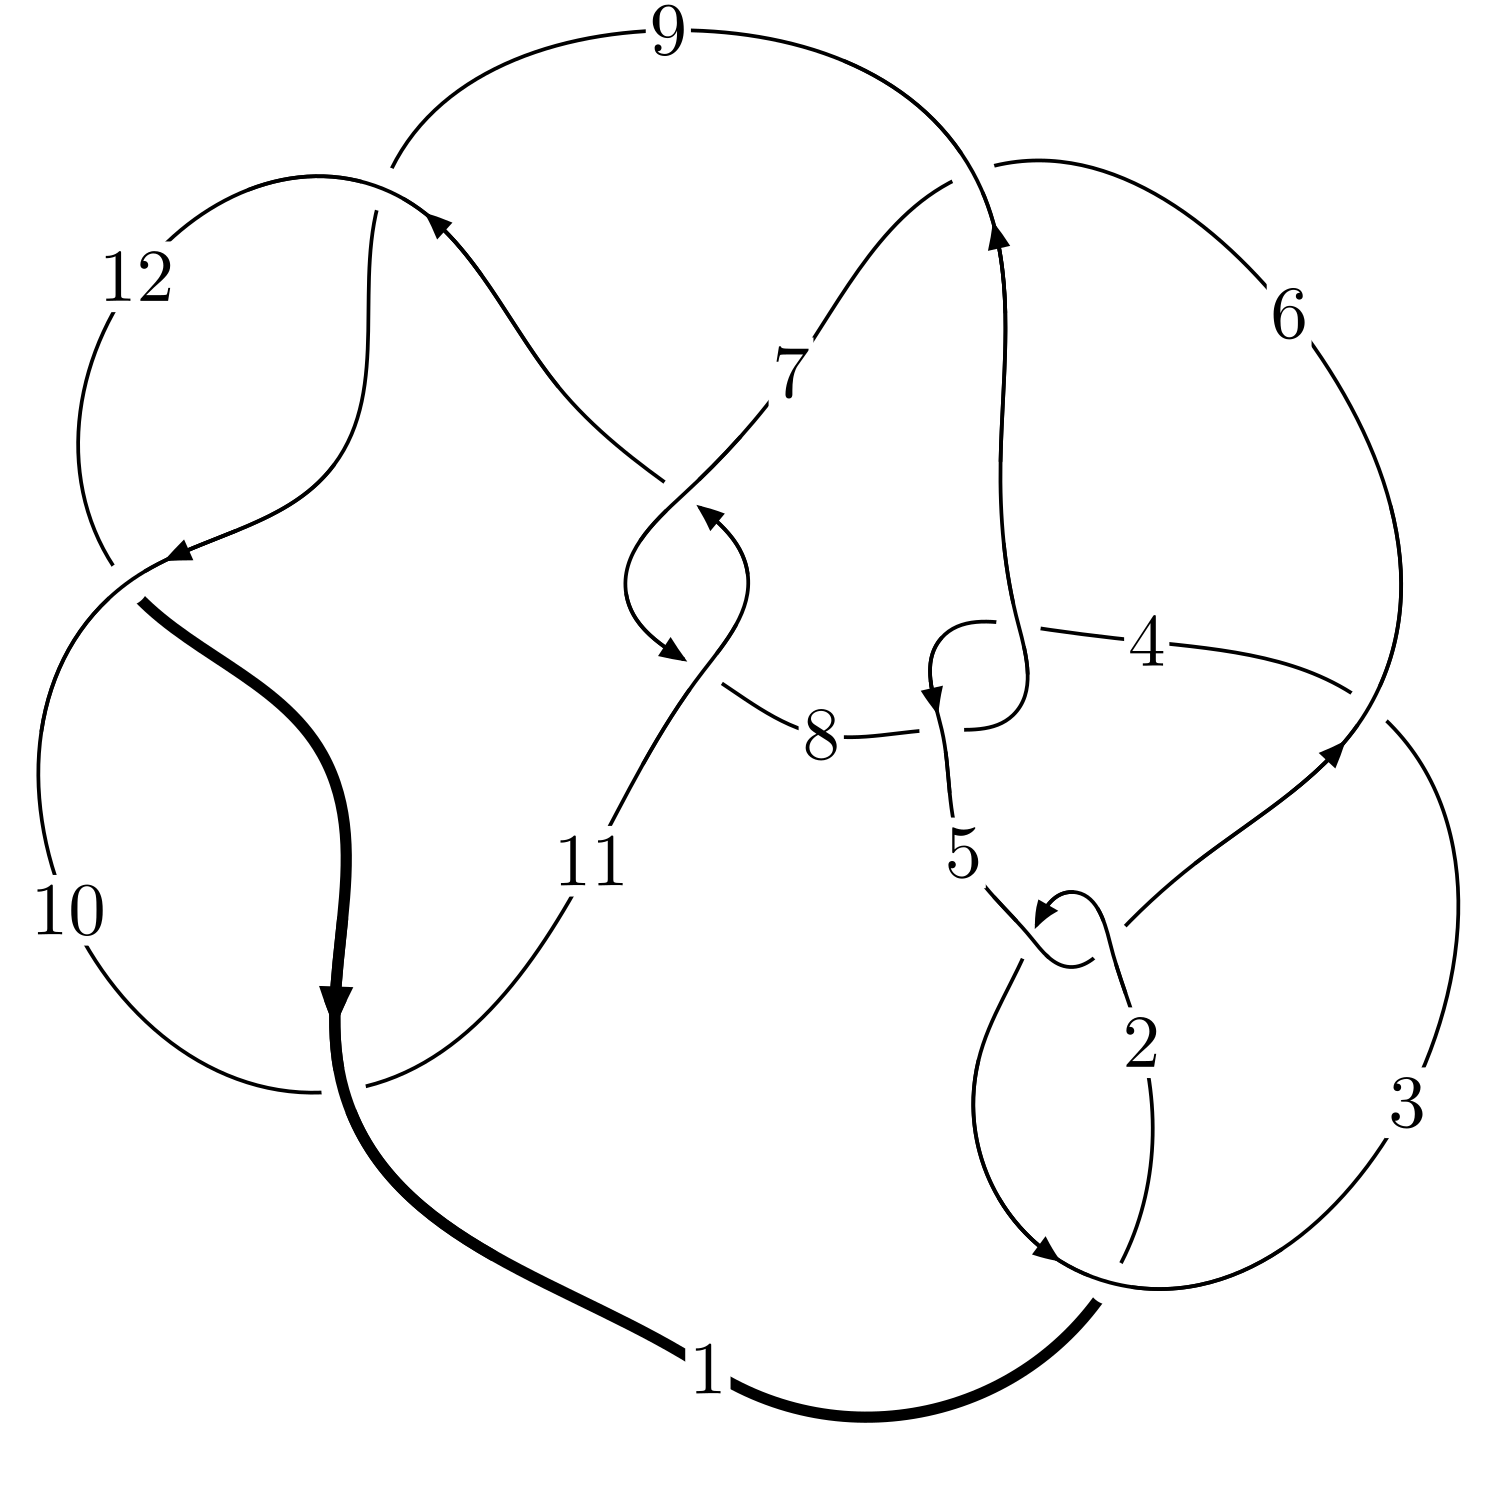
\includegraphics[width=112pt]{../../../GIT/diagram.site/Diagrams/png/2097_12n_0008.png}\\
\ \ \ A knot diagram\footnotemark}&
\allowdisplaybreaks
\textbf{Linearized knot diagam} \\
\cline{2-2}
 &
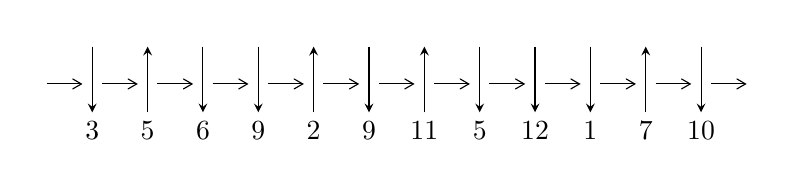
\begin{tikzpicture}[x=20pt, y=17pt]
	% nodes
	\node (C0) at (0, 0) {};
	\node (C1) at (1, 0) {};
	\node (C1U) at (1, +1) {};
	\node (C1D) at (1, -1) {3};

	\node (C2) at (2, 0) {};
	\node (C2U) at (2, +1) {};
	\node (C2D) at (2, -1) {5};

	\node (C3) at (3, 0) {};
	\node (C3U) at (3, +1) {};
	\node (C3D) at (3, -1) {6};

	\node (C4) at (4, 0) {};
	\node (C4U) at (4, +1) {};
	\node (C4D) at (4, -1) {9};

	\node (C5) at (5, 0) {};
	\node (C5U) at (5, +1) {};
	\node (C5D) at (5, -1) {2};

	\node (C6) at (6, 0) {};
	\node (C6U) at (6, +1) {};
	\node (C6D) at (6, -1) {9};

	\node (C7) at (7, 0) {};
	\node (C7U) at (7, +1) {};
	\node (C7D) at (7, -1) {11};

	\node (C8) at (8, 0) {};
	\node (C8U) at (8, +1) {};
	\node (C8D) at (8, -1) {5};

	\node (C9) at (9, 0) {};
	\node (C9U) at (9, +1) {};
	\node (C9D) at (9, -1) {12};

	\node (C10) at (10, 0) {};
	\node (C10U) at (10, +1) {};
	\node (C10D) at (10, -1) {1};

	\node (C11) at (11, 0) {};
	\node (C11U) at (11, +1) {};
	\node (C11D) at (11, -1) {7};

	\node (C12) at (12, 0) {};
	\node (C12U) at (12, +1) {};
	\node (C12D) at (12, -1) {10};
	\node (C13) at (13, 0) {};

	% arrows
	\draw[->,>={angle 60}]
	(C0) edge (C1) (C1) edge (C2) (C2) edge (C3) (C3) edge (C4) (C4) edge (C5) (C5) edge (C6) (C6) edge (C7) (C7) edge (C8) (C8) edge (C9) (C9) edge (C10) (C10) edge (C11) (C11) edge (C12) (C12) edge (C13) ;	\draw[->,>=stealth]
	(C1U) edge (C1D) (C2D) edge (C2U) (C3U) edge (C3D) (C4U) edge (C4D) (C5D) edge (C5U) (C6U) edge (C6D) (C7D) edge (C7U) (C8U) edge (C8D) (C9U) edge (C9D) (C10U) edge (C10D) (C11D) edge (C11U) (C12U) edge (C12D) ;
	\end{tikzpicture} \\
\hhline{~~} \\& 
\textbf{Solving Sequence} \\ \cline{2-2} 
 &
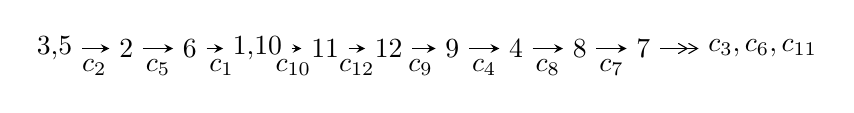
\begin{tikzpicture}[x=23pt, y=7pt]
	% node
	\node (A0) at (-1/8, 0) {3,5};
	\node (A1) at (1, 0) {2};
	\node (A2) at (2, 0) {6};
	\node (A3) at (49/16, 0) {1,10};
	\node (A4) at (33/8, 0) {11};
	\node (A5) at (41/8, 0) {12};
	\node (A6) at (49/8, 0) {9};
	\node (A7) at (57/8, 0) {4};
	\node (A8) at (65/8, 0) {8};
	\node (A9) at (73/8, 0) {7};
	\node (C1) at (1/2, -1) {$c_{2}$};
	\node (C2) at (3/2, -1) {$c_{5}$};
	\node (C3) at (5/2, -1) {$c_{1}$};
	\node (C4) at (29/8, -1) {$c_{10}$};
	\node (C5) at (37/8, -1) {$c_{12}$};
	\node (C6) at (45/8, -1) {$c_{9}$};
	\node (C7) at (53/8, -1) {$c_{4}$};
	\node (C8) at (61/8, -1) {$c_{8}$};
	\node (C9) at (69/8, -1) {$c_{7}$};
	\node (A10) at (11, 0) {$c_{3},c_{6},c_{11}$};

	% edge
	\draw[->,>=stealth]	
	(A0) edge (A1) (A1) edge (A2) (A2) edge (A3) (A3) edge (A4) (A4) edge (A5) (A5) edge (A6) (A6) edge (A7) (A7) edge (A8) (A8) edge (A9) ;
	\draw[->>,>={angle 60}]	
	(A9) edge (A10);
\end{tikzpicture} \\ 

\end{tabular} \\

\footnotetext{
The image of knot diagram is generated by the software ``\textbf{Draw programme}" developed by Andrew Bartholomew(\url{http://www.layer8.co.uk/maths/draw/index.htm\#Running-draw}), where we modified some parts for our purpose(\url{https://github.com/CATsTAILs/LinksPainter}).
}\phantom \\ \newline 
\centering \textbf{Ideals for irreducible components\footnotemark of $X_{\text{par}}$} 
 
\begin{align*}
I^u_{1}&=\langle 
-40170837860333 u^{44}+273898398784184 u^{43}+\cdots+57194726799376 b-67982681260688,\\
\phantom{I^u_{1}}&\phantom{= \langle  }19829193212635 u^{44}-141090112593855 u^{43}+\cdots+57194726799376 a+390935602889337,\\
\phantom{I^u_{1}}&\phantom{= \langle  }u^{45}-7 u^{44}+\cdots+13 u-1\rangle \\
I^u_{2}&=\langle 
-4 a^4 u-2 a^3 u-2 a^3+15 a^2+15 a u+5 b-3 u-3,\;a^5+4 a^3 u+4 a^3-5 a^2-2 a u+u+1,\;u^2+u+1\rangle \\
I^u_{3}&=\langle 
u^2+b- u+1,\;- u^4+u^3- u^2+a+1,\;u^5- u^4+2 u^3- u^2+u-1\rangle \\
\\
\end{align*}
\raggedright * 3 irreducible components of $\dim_{\mathbb{C}}=0$, with total 60 representations.\\
\footnotetext{All coefficients of polynomials are rational numbers. But the coefficients are sometimes approximated in decimal forms when there is not enough margin.}
\newpage
\renewcommand{\arraystretch}{1}
\centering \section*{I. $I^u_{1}= \langle -4.02\times10^{13} u^{44}+2.74\times10^{14} u^{43}+\cdots+5.72\times10^{13} b-6.80\times10^{13},\;1.98\times10^{13} u^{44}-1.41\times10^{14} u^{43}+\cdots+5.72\times10^{13} a+3.91\times10^{14},\;u^{45}-7 u^{44}+\cdots+13 u-1 \rangle$}
\flushleft \textbf{(i) Arc colorings}\\
\begin{tabular}{m{7pt} m{180pt} m{7pt} m{180pt} }
\flushright $a_{3}=$&$\begin{pmatrix}1\\0\end{pmatrix}$ \\
\flushright $a_{5}=$&$\begin{pmatrix}0\\u\end{pmatrix}$ \\
\flushright $a_{2}=$&$\begin{pmatrix}1\\u^2\end{pmatrix}$ \\
\flushright $a_{6}=$&$\begin{pmatrix}u\\u^3+u\end{pmatrix}$ \\
\flushright $a_{1}=$&$\begin{pmatrix}u^2+1\\u^2\end{pmatrix}$ \\
\flushright $a_{10}=$&$\begin{pmatrix}-0.346696 u^{44}+2.46684 u^{43}+\cdots+26.5461 u-6.83517\\0.702352 u^{44}-4.78888 u^{43}+\cdots-4.12647 u+1.18862\end{pmatrix}$ \\
\flushright $a_{11}=$&$\begin{pmatrix}-0.557267 u^{44}+3.84559 u^{43}+\cdots+30.7805 u-8.13179\\0.738824 u^{44}-5.11904 u^{43}+\cdots-4.10862 u+1.16824\end{pmatrix}$ \\
\flushright $a_{12}=$&$\begin{pmatrix}0.948786 u^{44}-6.63640 u^{43}+\cdots-38.0499 u+9.08094\\-0.352063 u^{44}+2.54967 u^{43}+\cdots+10.9763 u-1.85015\end{pmatrix}$ \\
\flushright $a_{9}=$&$\begin{pmatrix}1.14775 u^{44}-8.03211 u^{43}+\cdots-29.6955 u+4.33683\\-0.0391055 u^{44}+0.648251 u^{43}+\cdots+12.0682 u-1.19731\end{pmatrix}$ \\
\flushright $a_{4}=$&$\begin{pmatrix}u^4+u^2+1\\u^6+2 u^4+u^2\end{pmatrix}$ \\
\flushright $a_{8}=$&$\begin{pmatrix}1.14775 u^{44}-8.03211 u^{43}+\cdots-29.6955 u+4.33683\\0.256025 u^{44}-1.48232 u^{43}+\cdots+10.9482 u-1.19944\end{pmatrix}$ \\
\flushright $a_{7}=$&$\begin{pmatrix}- u^2-1\\\frac{1}{16} u^{43}-\frac{3}{8} u^{42}+\cdots+\frac{11}{4} u-\frac{1}{16}\end{pmatrix}$\\&\end{tabular}
\flushleft \textbf{(ii) Obstruction class $= -1$}\\~\\
\flushleft \textbf{(iii) Cusp Shapes $= \frac{60972380652257}{57194726799376} u^{44}-\frac{218749636382387}{28597363399688} u^{43}+\cdots+\frac{1862967060953113}{57194726799376} u-\frac{208231471984261}{28597363399688}$}\\~\\
\newpage\renewcommand{\arraystretch}{1}
\flushleft \textbf{(iv) u-Polynomials at the component}\newline \\
\begin{tabular}{m{50pt}|m{274pt}}
Crossings & \hspace{64pt}u-Polynomials at each crossing \\
\hline $$\begin{aligned}c_{1}\end{aligned}$$&$\begin{aligned}
&u^{45}+29 u^{44}+\cdots+23 u-1
\end{aligned}$\\
\hline $$\begin{aligned}c_{2},c_{5}\end{aligned}$$&$\begin{aligned}
&u^{45}+7 u^{44}+\cdots+13 u+1
\end{aligned}$\\
\hline $$\begin{aligned}c_{3}\end{aligned}$$&$\begin{aligned}
&u^{45}-7 u^{44}+\cdots+3 u+1
\end{aligned}$\\
\hline $$\begin{aligned}c_{4},c_{8}\end{aligned}$$&$\begin{aligned}
&u^{45}+2 u^{44}+\cdots+3072 u^2-1024
\end{aligned}$\\
\hline $$\begin{aligned}c_{6}\end{aligned}$$&$\begin{aligned}
&u^{45}-4 u^{44}+\cdots+2 u-1
\end{aligned}$\\
\hline $$\begin{aligned}c_{7},c_{11}\end{aligned}$$&$\begin{aligned}
&u^{45}-3 u^{44}+\cdots+32 u-32
\end{aligned}$\\
\hline $$\begin{aligned}c_{9},c_{10},c_{12}\end{aligned}$$&$\begin{aligned}
&u^{45}-8 u^{44}+\cdots-8 u-1
\end{aligned}$\\
\hline
\end{tabular}\\~\\
\newpage\renewcommand{\arraystretch}{1}
\flushleft \textbf{(v) Riley Polynomials at the component}\newline \\
\begin{tabular}{m{50pt}|m{274pt}}
Crossings & \hspace{64pt}Riley Polynomials at each crossing \\
\hline $$\begin{aligned}c_{1}\end{aligned}$$&$\begin{aligned}
&y^{45}-19 y^{44}+\cdots+3799 y-1
\end{aligned}$\\
\hline $$\begin{aligned}c_{2},c_{5}\end{aligned}$$&$\begin{aligned}
&y^{45}+29 y^{44}+\cdots+23 y-1
\end{aligned}$\\
\hline $$\begin{aligned}c_{3}\end{aligned}$$&$\begin{aligned}
&y^{45}-67 y^{44}+\cdots+23 y-1
\end{aligned}$\\
\hline $$\begin{aligned}c_{4},c_{8}\end{aligned}$$&$\begin{aligned}
&y^{45}-60 y^{44}+\cdots+6291456 y-1048576
\end{aligned}$\\
\hline $$\begin{aligned}c_{6}\end{aligned}$$&$\begin{aligned}
&y^{45}-62 y^{44}+\cdots+14 y-1
\end{aligned}$\\
\hline $$\begin{aligned}c_{7},c_{11}\end{aligned}$$&$\begin{aligned}
&y^{45}+39 y^{44}+\cdots-4608 y-1024
\end{aligned}$\\
\hline $$\begin{aligned}c_{9},c_{10},c_{12}\end{aligned}$$&$\begin{aligned}
&y^{45}-50 y^{44}+\cdots+70 y^2-1
\end{aligned}$\\
\hline
\end{tabular}\\~\\
\newpage\flushleft \textbf{(vi) Complex Volumes and Cusp Shapes}
$$\begin{array}{c|c|c}  
\text{Solutions to }I^u_{1}& \I (\text{vol} + \sqrt{-1}CS) & \text{Cusp shape}\\
 \hline 
\begin{aligned}
u &= -0.448428 + 0.886782 I \\
a &= \phantom{-}3.29054 - 2.26057 I \\
b &= -0.04313 - 3.34261 I\end{aligned}
 & -1.93664 - 1.84719 I & \phantom{-}16.6318 + 21.5784 I \\ \hline\begin{aligned}
u &= -0.448428 - 0.886782 I \\
a &= \phantom{-}3.29054 + 2.26057 I \\
b &= -0.04313 + 3.34261 I\end{aligned}
 & -1.93664 + 1.84719 I & \phantom{-}16.6318 - 21.5784 I \\ \hline\begin{aligned}
u &= \phantom{-}1.028510 + 0.052980 I \\
a &= \phantom{-}0.875035 - 0.619833 I \\
b &= \phantom{-}0.792997 + 0.140103 I\end{aligned}
 & -8.08739 - 3.08320 I & -6.91743 + 2.52914 I \\ \hline\begin{aligned}
u &= \phantom{-}1.028510 - 0.052980 I \\
a &= \phantom{-}0.875035 + 0.619833 I \\
b &= \phantom{-}0.792997 - 0.140103 I\end{aligned}
 & -8.08739 + 3.08320 I & -6.91743 - 2.52914 I \\ \hline\begin{aligned}
u &= \phantom{-}0.141103 + 1.020830 I \\
a &= \phantom{-}0.123326 - 0.575048 I \\
b &= -0.602098 - 0.954633 I\end{aligned}
 & -1.88299 + 2.68710 I & -8.64703 - 3.04236 I \\ \hline\begin{aligned}
u &= \phantom{-}0.141103 - 1.020830 I \\
a &= \phantom{-}0.123326 + 0.575048 I \\
b &= -0.602098 + 0.954633 I\end{aligned}
 & -1.88299 - 2.68710 I & -8.64703 + 3.04236 I \\ \hline\begin{aligned}
u &= \phantom{-}1.04389\phantom{ +0.000000I} \\
a &= \phantom{-}3.48098\phantom{ +0.000000I} \\
b &= \phantom{-}2.56398\phantom{ +0.000000I}\end{aligned}
 & -10.3675\phantom{ +0.000000I} & -7.74840\phantom{ +0.000000I} \\ \hline\begin{aligned}
u &= -0.814101 + 0.473442 I \\
a &= -1.85931 - 0.05637 I \\
b &= -1.69396 + 0.05742 I\end{aligned}
 & -6.36217 - 1.58930 I & -8.13248 + 2.19731 I \\ \hline\begin{aligned}
u &= -0.814101 - 0.473442 I \\
a &= -1.85931 + 0.05637 I \\
b &= -1.69396 - 0.05742 I\end{aligned}
 & -6.36217 + 1.58930 I & -8.13248 - 2.19731 I \\ \hline\begin{aligned}
u &= \phantom{-}0.321638 + 1.027370 I \\
a &= -0.357029 - 0.516807 I \\
b &= \phantom{-}0.721264 + 1.082480 I\end{aligned}
 & -6.92269 + 6.44252 I & -13.9889 - 5.4327 I\\
 \hline 
 \end{array}$$\newpage$$\begin{array}{c|c|c}  
\text{Solutions to }I^u_{1}& \I (\text{vol} + \sqrt{-1}CS) & \text{Cusp shape}\\
 \hline 
\begin{aligned}
u &= \phantom{-}0.321638 - 1.027370 I \\
a &= -0.357029 + 0.516807 I \\
b &= \phantom{-}0.721264 - 1.082480 I\end{aligned}
 & -6.92269 - 6.44252 I & -13.9889 + 5.4327 I \\ \hline\begin{aligned}
u &= \phantom{-}1.074090 + 0.154235 I \\
a &= -2.72392 + 0.96068 I \\
b &= -2.30814 + 0.29423 I\end{aligned}
 & -15.4421 - 7.7641 I & -8.55026 + 3.19844 I \\ \hline\begin{aligned}
u &= \phantom{-}1.074090 - 0.154235 I \\
a &= -2.72392 - 0.96068 I \\
b &= -2.30814 - 0.29423 I\end{aligned}
 & -15.4421 + 7.7641 I & -8.55026 - 3.19844 I \\ \hline\begin{aligned}
u &= -0.558842 + 0.933277 I \\
a &= -1.240750 - 0.138767 I \\
b &= -0.96715 + 1.42473 I\end{aligned}
 & -0.77833 - 2.85163 I & -9.27214 + 0. I\phantom{ +0.000000I} \\ \hline\begin{aligned}
u &= -0.558842 - 0.933277 I \\
a &= -1.240750 + 0.138767 I \\
b &= -0.96715 - 1.42473 I\end{aligned}
 & -0.77833 + 2.85163 I & -9.27214 + 0. I\phantom{ +0.000000I} \\ \hline\begin{aligned}
u &= \phantom{-}0.038638 + 1.093140 I \\
a &= \phantom{-}0.764813 - 0.243323 I \\
b &= -1.73664 - 1.54360 I\end{aligned}
 & -4.80137 + 0.66249 I & -10.84717 + 0. I\phantom{ +0.000000I} \\ \hline\begin{aligned}
u &= \phantom{-}0.038638 - 1.093140 I \\
a &= \phantom{-}0.764813 + 0.243323 I \\
b &= -1.73664 + 1.54360 I\end{aligned}
 & -4.80137 - 0.66249 I & -10.84717 + 0. I\phantom{ +0.000000I} \\ \hline\begin{aligned}
u &= -0.095599 + 1.102010 I \\
a &= \phantom{-}0.691464 + 0.377467 I \\
b &= -0.104979 + 0.147687 I\end{aligned}
 & -3.59727 - 1.96898 I & -11.38503 + 2.89411 I \\ \hline\begin{aligned}
u &= -0.095599 - 1.102010 I \\
a &= \phantom{-}0.691464 - 0.377467 I \\
b &= -0.104979 - 0.147687 I\end{aligned}
 & -3.59727 + 1.96898 I & -11.38503 - 2.89411 I \\ \hline\begin{aligned}
u &= -0.464257 + 0.743525 I \\
a &= -0.128607 + 0.894701 I \\
b &= \phantom{-}0.879012 + 0.408581 I\end{aligned}
 & -0.10245 - 1.42024 I & -3.50008 + 5.75375 I\\
 \hline 
 \end{array}$$\newpage$$\begin{array}{c|c|c}  
\text{Solutions to }I^u_{1}& \I (\text{vol} + \sqrt{-1}CS) & \text{Cusp shape}\\
 \hline 
\begin{aligned}
u &= -0.464257 - 0.743525 I \\
a &= -0.128607 - 0.894701 I \\
b &= \phantom{-}0.879012 - 0.408581 I\end{aligned}
 & -0.10245 + 1.42024 I & -3.50008 - 5.75375 I \\ \hline\begin{aligned}
u &= \phantom{-}0.840032\phantom{ +0.000000I} \\
a &= -1.01212\phantom{ +0.000000I} \\
b &= -0.718511\phantom{ +0.000000I}\end{aligned}
 & -3.18298\phantom{ +0.000000I} & \phantom{-}0.134470\phantom{ +0.000000I} \\ \hline\begin{aligned}
u &= -0.209858 + 0.761572 I \\
a &= -0.588066 + 0.563430 I \\
b &= \phantom{-}0.557407 + 0.666651 I\end{aligned}
 & -0.270200 - 1.317790 I & -2.14262 + 3.99951 I \\ \hline\begin{aligned}
u &= -0.209858 - 0.761572 I \\
a &= -0.588066 - 0.563430 I \\
b &= \phantom{-}0.557407 - 0.666651 I\end{aligned}
 & -0.270200 + 1.317790 I & -2.14262 - 3.99951 I \\ \hline\begin{aligned}
u &= -0.715937 + 1.055430 I \\
a &= \phantom{-}0.47884 + 1.81232 I \\
b &= \phantom{-}1.310670 + 0.236185 I\end{aligned}
 & -7.98005 - 4.06553 I & \phantom{-0.000000 } 0 \\ \hline\begin{aligned}
u &= -0.715937 - 1.055430 I \\
a &= \phantom{-}0.47884 - 1.81232 I \\
b &= \phantom{-}1.310670 - 0.236185 I\end{aligned}
 & -7.98005 + 4.06553 I & \phantom{-0.000000 } 0 \\ \hline\begin{aligned}
u &= \phantom{-}0.414289 + 0.552563 I \\
a &= -0.545658 - 0.831909 I \\
b &= -0.997622 + 0.175155 I\end{aligned}
 & -5.50892 - 3.28114 I & -8.73853 + 6.07709 I \\ \hline\begin{aligned}
u &= \phantom{-}0.414289 - 0.552563 I \\
a &= -0.545658 + 0.831909 I \\
b &= -0.997622 - 0.175155 I\end{aligned}
 & -5.50892 + 3.28114 I & -8.73853 - 6.07709 I \\ \hline\begin{aligned}
u &= \phantom{-}0.456920 + 1.233790 I \\
a &= \phantom{-}0.146367 - 0.696106 I \\
b &= \phantom{-}0.998812 - 0.254559 I\end{aligned}
 & -6.87697 + 4.62897 I & \phantom{-0.000000 } 0 \\ \hline\begin{aligned}
u &= \phantom{-}0.456920 - 1.233790 I \\
a &= \phantom{-}0.146367 + 0.696106 I \\
b &= \phantom{-}0.998812 + 0.254559 I\end{aligned}
 & -6.87697 - 4.62897 I & \phantom{-0.000000 } 0\\
 \hline 
 \end{array}$$\newpage$$\begin{array}{c|c|c}  
\text{Solutions to }I^u_{1}& \I (\text{vol} + \sqrt{-1}CS) & \text{Cusp shape}\\
 \hline 
\begin{aligned}
u &= -0.236201 + 1.315500 I \\
a &= \phantom{-}0.223845 + 0.997497 I \\
b &= \phantom{-}2.56560 + 0.53987 I\end{aligned}
 & -11.96940 - 4.68670 I & \phantom{-0.000000 } 0 \\ \hline\begin{aligned}
u &= -0.236201 - 1.315500 I \\
a &= \phantom{-}0.223845 - 0.997497 I \\
b &= \phantom{-}2.56560 - 0.53987 I\end{aligned}
 & -11.96940 + 4.68670 I & \phantom{-0.000000 } 0 \\ \hline\begin{aligned}
u &= \phantom{-}0.53792 + 1.32330 I \\
a &= -0.520780 + 0.416398 I \\
b &= -1.64420 + 0.02216 I\end{aligned}
 & -12.0273 + 8.6721 I & \phantom{-0.000000 } 0 \\ \hline\begin{aligned}
u &= \phantom{-}0.53792 - 1.32330 I \\
a &= -0.520780 - 0.416398 I \\
b &= -1.64420 - 0.02216 I\end{aligned}
 & -12.0273 - 8.6721 I & \phantom{-0.000000 } 0 \\ \hline\begin{aligned}
u &= \phantom{-}0.47555 + 1.35442 I \\
a &= \phantom{-}0.116010 + 0.860979 I \\
b &= -0.012680 + 0.444909 I\end{aligned}
 & -12.52320 + 2.24438 I & \phantom{-0.000000 } 0 \\ \hline\begin{aligned}
u &= \phantom{-}0.47555 - 1.35442 I \\
a &= \phantom{-}0.116010 - 0.860979 I \\
b &= -0.012680 - 0.444909 I\end{aligned}
 & -12.52320 - 2.24438 I & \phantom{-0.000000 } 0 \\ \hline\begin{aligned}
u &= \phantom{-}0.60027 + 1.30875 I \\
a &= \phantom{-}1.41525 - 1.67542 I \\
b &= \phantom{-}3.06355 - 0.12659 I\end{aligned}
 & -19.0180 + 13.7371 I & \phantom{-0.000000 } 0 \\ \hline\begin{aligned}
u &= \phantom{-}0.60027 - 1.30875 I \\
a &= \phantom{-}1.41525 + 1.67542 I \\
b &= \phantom{-}3.06355 + 0.12659 I\end{aligned}
 & -19.0180 - 13.7371 I & \phantom{-0.000000 } 0 \\ \hline\begin{aligned}
u &= \phantom{-}0.51317 + 1.34856 I \\
a &= -0.98613 + 2.21993 I \\
b &= -3.05558 + 1.18362 I\end{aligned}
 & -14.5875 + 5.5390 I & \phantom{-0.000000 } 0 \\ \hline\begin{aligned}
u &= \phantom{-}0.51317 - 1.34856 I \\
a &= -0.98613 - 2.21993 I \\
b &= -3.05558 - 1.18362 I\end{aligned}
 & -14.5875 - 5.5390 I & \phantom{-0.000000 } 0\\
 \hline 
 \end{array}$$\newpage$$\begin{array}{c|c|c}  
\text{Solutions to }I^u_{1}& \I (\text{vol} + \sqrt{-1}CS) & \text{Cusp shape}\\
 \hline 
\begin{aligned}
u &= \phantom{-}0.40664 + 1.42221 I \\
a &= \phantom{-}0.22163 - 1.91263 I \\
b &= \phantom{-}1.91377 - 1.51963 I\end{aligned}
 & \phantom{-}18.8970 - 2.5007 I & \phantom{-0.000000 } 0 \\ \hline\begin{aligned}
u &= \phantom{-}0.40664 - 1.42221 I \\
a &= \phantom{-}0.22163 + 1.91263 I \\
b &= \phantom{-}1.91377 + 1.51963 I\end{aligned}
 & \phantom{-}18.8970 + 2.5007 I & \phantom{-0.000000 } 0 \\ \hline\begin{aligned}
u &= \phantom{-}0.027627 + 0.285904 I \\
a &= -1.54121 + 0.47713 I \\
b &= \phantom{-}0.419324 + 0.349696 I\end{aligned}
 & -0.299097 - 1.132870 I & -4.25483 + 6.05161 I \\ \hline\begin{aligned}
u &= \phantom{-}0.027627 - 0.285904 I \\
a &= -1.54121 - 0.47713 I \\
b &= \phantom{-}0.419324 - 0.349696 I\end{aligned}
 & -0.299097 + 1.132870 I & -4.25483 - 6.05161 I \\ \hline\begin{aligned}
u &= \phantom{-}0.129774\phantom{ +0.000000I} \\
a &= -5.18021\phantom{ +0.000000I} \\
b &= \phantom{-}1.04208\phantom{ +0.000000I}\end{aligned}
 & -2.19508\phantom{ +0.000000I} & -3.54080\phantom{ +0.000000I}\\
 \hline 
 \end{array}$$\newpage\newpage\renewcommand{\arraystretch}{1}
\centering \section*{II. $I^u_{2}= \langle -4 a^4 u-2 a^3 u+\cdots+15 a^2-3,\;a^5+4 a^3 u+4 a^3-5 a^2-2 a u+u+1,\;u^2+u+1 \rangle$}
\flushleft \textbf{(i) Arc colorings}\\
\begin{tabular}{m{7pt} m{180pt} m{7pt} m{180pt} }
\flushright $a_{3}=$&$\begin{pmatrix}1\\0\end{pmatrix}$ \\
\flushright $a_{5}=$&$\begin{pmatrix}0\\u\end{pmatrix}$ \\
\flushright $a_{2}=$&$\begin{pmatrix}1\\- u-1\end{pmatrix}$ \\
\flushright $a_{6}=$&$\begin{pmatrix}u\\u+1\end{pmatrix}$ \\
\flushright $a_{1}=$&$\begin{pmatrix}- u\\- u-1\end{pmatrix}$ \\
\flushright $a_{10}=$&$\begin{pmatrix}a\\\frac{4}{5} a^4 u+\frac{2}{5} a^3 u+\cdots-3 a^2+\frac{3}{5}\end{pmatrix}$ \\
\flushright $a_{11}=$&$\begin{pmatrix}-\frac{4}{5} a^4+\frac{2}{5} a^3 u-3 a^2 u-3 a^2+3 a+\frac{3}{5} u\\\frac{8}{5} a^4 u+\frac{4}{5} a^3 u+\cdots-6 a^2+\frac{6}{5}\end{pmatrix}$ \\
\flushright $a_{12}=$&$\begin{pmatrix}-\frac{2}{5} a^4+\frac{1}{5} a^3 u-2 a^2 u-2 a^2+a-\frac{1}{5} u\\-\frac{1}{5} a^4 u-\frac{3}{5} a^3 u+\cdots-\frac{3}{5} a^3-\frac{2}{5}\end{pmatrix}$ \\
\flushright $a_{9}=$&$\begin{pmatrix}0\\-\frac{1}{5} a^4 u-\frac{3}{5} a^3 u+\cdots-\frac{3}{5} a^3-\frac{2}{5}\end{pmatrix}$ \\
\flushright $a_{4}=$&$\begin{pmatrix}0\\u\end{pmatrix}$ \\
\flushright $a_{8}=$&$\begin{pmatrix}0\\-\frac{1}{5} a^4 u-\frac{3}{5} a^3 u+\cdots-\frac{3}{5} a^3-\frac{2}{5}\end{pmatrix}$ \\
\flushright $a_{7}=$&$\begin{pmatrix}u\\-\frac{2}{5} a^4 u-\frac{6}{5} a^3 u+\cdots-\frac{6}{5} a^3+\frac{6}{5}\end{pmatrix}$\\&\end{tabular}
\flushleft \textbf{(ii) Obstruction class $= 1$}\\~\\
\flushleft \textbf{(iii) Cusp Shapes $= -\frac{14}{5} a^4 u-3 a^4-\frac{7}{5} a^3 u-\frac{2}{5} a^3-15 a^2 u-3 a^2+11 a u+16 a+\frac{27}{5} u-\frac{33}{5}$}\\~\\
\newpage\renewcommand{\arraystretch}{1}
\flushleft \textbf{(iv) u-Polynomials at the component}\newline \\
\begin{tabular}{m{50pt}|m{274pt}}
Crossings & \hspace{64pt}u-Polynomials at each crossing \\
\hline $$\begin{aligned}c_{1},c_{3},c_{5}\end{aligned}$$&$\begin{aligned}
&(u^2- u+1)^5
\end{aligned}$\\
\hline $$\begin{aligned}c_{2}\end{aligned}$$&$\begin{aligned}
&(u^2+u+1)^5
\end{aligned}$\\
\hline $$\begin{aligned}c_{4},c_{8}\end{aligned}$$&$\begin{aligned}
&u^{10}
\end{aligned}$\\
\hline $$\begin{aligned}c_{6}\end{aligned}$$&$\begin{aligned}
&(u^5-3 u^4+4 u^3- u^2- u+1)^2
\end{aligned}$\\
\hline $$\begin{aligned}c_{7}\end{aligned}$$&$\begin{aligned}
&(u^5- u^4+2 u^3- u^2+u-1)^2
\end{aligned}$\\
\hline $$\begin{aligned}c_{9},c_{10}\end{aligned}$$&$\begin{aligned}
&(u^5+u^4-2 u^3- u^2+u-1)^2
\end{aligned}$\\
\hline $$\begin{aligned}c_{11}\end{aligned}$$&$\begin{aligned}
&(u^5+u^4+2 u^3+u^2+u+1)^2
\end{aligned}$\\
\hline $$\begin{aligned}c_{12}\end{aligned}$$&$\begin{aligned}
&(u^5- u^4-2 u^3+u^2+u+1)^2
\end{aligned}$\\
\hline
\end{tabular}\\~\\
\newpage\renewcommand{\arraystretch}{1}
\flushleft \textbf{(v) Riley Polynomials at the component}\newline \\
\begin{tabular}{m{50pt}|m{274pt}}
Crossings & \hspace{64pt}Riley Polynomials at each crossing \\
\hline $$\begin{aligned}c_{1},c_{2},c_{3}\\c_{5}\end{aligned}$$&$\begin{aligned}
&(y^2+y+1)^5
\end{aligned}$\\
\hline $$\begin{aligned}c_{4},c_{8}\end{aligned}$$&$\begin{aligned}
&y^{10}
\end{aligned}$\\
\hline $$\begin{aligned}c_{6}\end{aligned}$$&$\begin{aligned}
&(y^5- y^4+8 y^3-3 y^2+3 y-1)^2
\end{aligned}$\\
\hline $$\begin{aligned}c_{7},c_{11}\end{aligned}$$&$\begin{aligned}
&(y^5+3 y^4+4 y^3+y^2- y-1)^2
\end{aligned}$\\
\hline $$\begin{aligned}c_{9},c_{10},c_{12}\end{aligned}$$&$\begin{aligned}
&(y^5-5 y^4+8 y^3-3 y^2- y-1)^2
\end{aligned}$\\
\hline
\end{tabular}\\~\\
\newpage\flushleft \textbf{(vi) Complex Volumes and Cusp Shapes}
$$\begin{array}{c|c|c}  
\text{Solutions to }I^u_{2}& \I (\text{vol} + \sqrt{-1}CS) & \text{Cusp shape}\\
 \hline 
\begin{aligned}
u &= -0.500000 + 0.866025 I \\
a &= \phantom{-}1.012010 - 0.734701 I \\
b &= \phantom{-}0.768927 - 0.124653 I\end{aligned}
 & -5.87256 + 2.37095 I & -11.57979 + 0.88917 I \\ \hline\begin{aligned}
u &= -0.500000 + 0.866025 I \\
a &= \phantom{-}0.130268 - 1.243770 I \\
b &= -0.492416 + 0.603584 I\end{aligned}
 & -5.87256 - 6.43072 I & -6.27578 + 5.55522 I \\ \hline\begin{aligned}
u &= -0.500000 + 0.866025 I \\
a &= -0.364485 - 0.347423 I \\
b &= -1.114310 + 0.148503 I\end{aligned}
 & -0.329100 - 0.499304 I & -6.44749 - 1.44665 I \\ \hline\begin{aligned}
u &= -0.500000 + 0.866025 I \\
a &= \phantom{-}0.483119 + 0.141942 I \\
b &= \phantom{-}0.685764 - 0.890773 I\end{aligned}
 & -0.32910 - 3.56046 I & -2.59686 + 8.38554 I \\ \hline\begin{aligned}
u &= -0.500000 + 0.866025 I \\
a &= -1.26091 + 2.18395 I \\
b &= \phantom{-}0.652039 + 1.129360 I\end{aligned}
 & -2.40108 - 2.02988 I & -7.10008 + 5.66929 I \\ \hline\begin{aligned}
u &= -0.500000 - 0.866025 I \\
a &= \phantom{-}1.012010 + 0.734701 I \\
b &= \phantom{-}0.768927 + 0.124653 I\end{aligned}
 & -5.87256 - 2.37095 I & -11.57979 - 0.88917 I \\ \hline\begin{aligned}
u &= -0.500000 - 0.866025 I \\
a &= \phantom{-}0.130268 + 1.243770 I \\
b &= -0.492416 - 0.603584 I\end{aligned}
 & -5.87256 + 6.43072 I & -6.27578 - 5.55522 I \\ \hline\begin{aligned}
u &= -0.500000 - 0.866025 I \\
a &= -0.364485 + 0.347423 I \\
b &= -1.114310 - 0.148503 I\end{aligned}
 & -0.329100 + 0.499304 I & -6.44749 + 1.44665 I \\ \hline\begin{aligned}
u &= -0.500000 - 0.866025 I \\
a &= \phantom{-}0.483119 - 0.141942 I \\
b &= \phantom{-}0.685764 + 0.890773 I\end{aligned}
 & -0.32910 + 3.56046 I & -2.59686 - 8.38554 I \\ \hline\begin{aligned}
u &= -0.500000 - 0.866025 I \\
a &= -1.26091 - 2.18395 I \\
b &= \phantom{-}0.652039 - 1.129360 I\end{aligned}
 & -2.40108 + 2.02988 I & -7.10008 - 5.66929 I\\
 \hline 
 \end{array}$$\newpage\newpage\renewcommand{\arraystretch}{1}
\centering \section*{III. $I^u_{3}= \langle u^2+b- u+1,\;- u^4+u^3- u^2+a+1,\;u^5- u^4+2 u^3- u^2+u-1 \rangle$}
\flushleft \textbf{(i) Arc colorings}\\
\begin{tabular}{m{7pt} m{180pt} m{7pt} m{180pt} }
\flushright $a_{3}=$&$\begin{pmatrix}1\\0\end{pmatrix}$ \\
\flushright $a_{5}=$&$\begin{pmatrix}0\\u\end{pmatrix}$ \\
\flushright $a_{2}=$&$\begin{pmatrix}1\\u^2\end{pmatrix}$ \\
\flushright $a_{6}=$&$\begin{pmatrix}u\\u^3+u\end{pmatrix}$ \\
\flushright $a_{1}=$&$\begin{pmatrix}u^2+1\\u^2\end{pmatrix}$ \\
\flushright $a_{10}=$&$\begin{pmatrix}u^4- u^3+u^2-1\\- u^2+u-1\end{pmatrix}$ \\
\flushright $a_{11}=$&$\begin{pmatrix}u^4- u^3+2 u^2\\u-1\end{pmatrix}$ \\
\flushright $a_{12}=$&$\begin{pmatrix}u^4- u^3+2 u^2\\u-1\end{pmatrix}$ \\
\flushright $a_{9}=$&$\begin{pmatrix}- u^2-1\\- u^2\end{pmatrix}$ \\
\flushright $a_{4}=$&$\begin{pmatrix}u^4+u^2+1\\u^4- u^3+u^2+1\end{pmatrix}$ \\
\flushright $a_{8}=$&$\begin{pmatrix}- u^2-1\\u^4\end{pmatrix}$ \\
\flushright $a_{7}=$&$\begin{pmatrix}- u^2-1\\u^4\end{pmatrix}$\\&\end{tabular}
\flushleft \textbf{(ii) Obstruction class $= 1$}\\~\\
\flushleft \textbf{(iii) Cusp Shapes $= -3 u^4+5 u^3-4 u^2-9$}\\~\\
\newpage\renewcommand{\arraystretch}{1}
\flushleft \textbf{(iv) u-Polynomials at the component}\newline \\
\begin{tabular}{m{50pt}|m{274pt}}
Crossings & \hspace{64pt}u-Polynomials at each crossing \\
\hline $$\begin{aligned}c_{1}\end{aligned}$$&$\begin{aligned}
&u^5-3 u^4+4 u^3- u^2- u+1
\end{aligned}$\\
\hline $$\begin{aligned}c_{2}\end{aligned}$$&$\begin{aligned}
&u^5- u^4+2 u^3- u^2+u-1
\end{aligned}$\\
\hline $$\begin{aligned}c_{3},c_{4}\end{aligned}$$&$\begin{aligned}
&u^5+u^4-2 u^3- u^2+u-1
\end{aligned}$\\
\hline $$\begin{aligned}c_{5}\end{aligned}$$&$\begin{aligned}
&u^5+u^4+2 u^3+u^2+u+1
\end{aligned}$\\
\hline $$\begin{aligned}c_{6}\end{aligned}$$&$\begin{aligned}
&u^5-5 u^4+8 u^3-3 u^2- u-1
\end{aligned}$\\
\hline $$\begin{aligned}c_{7},c_{11}\end{aligned}$$&$\begin{aligned}
&u^5
\end{aligned}$\\
\hline $$\begin{aligned}c_{8}\end{aligned}$$&$\begin{aligned}
&u^5- u^4-2 u^3+u^2+u+1
\end{aligned}$\\
\hline $$\begin{aligned}c_{9},c_{10}\end{aligned}$$&$\begin{aligned}
&(u-1)^5
\end{aligned}$\\
\hline $$\begin{aligned}c_{12}\end{aligned}$$&$\begin{aligned}
&(u+1)^5
\end{aligned}$\\
\hline
\end{tabular}\\~\\
\newpage\renewcommand{\arraystretch}{1}
\flushleft \textbf{(v) Riley Polynomials at the component}\newline \\
\begin{tabular}{m{50pt}|m{274pt}}
Crossings & \hspace{64pt}Riley Polynomials at each crossing \\
\hline $$\begin{aligned}c_{1}\end{aligned}$$&$\begin{aligned}
&y^5- y^4+8 y^3-3 y^2+3 y-1
\end{aligned}$\\
\hline $$\begin{aligned}c_{2},c_{5}\end{aligned}$$&$\begin{aligned}
&y^5+3 y^4+4 y^3+y^2- y-1
\end{aligned}$\\
\hline $$\begin{aligned}c_{3},c_{4},c_{8}\end{aligned}$$&$\begin{aligned}
&y^5-5 y^4+8 y^3-3 y^2- y-1
\end{aligned}$\\
\hline $$\begin{aligned}c_{6}\end{aligned}$$&$\begin{aligned}
&y^5-9 y^4+32 y^3-35 y^2-5 y-1
\end{aligned}$\\
\hline $$\begin{aligned}c_{7},c_{11}\end{aligned}$$&$\begin{aligned}
&y^5
\end{aligned}$\\
\hline $$\begin{aligned}c_{9},c_{10},c_{12}\end{aligned}$$&$\begin{aligned}
&(y-1)^5
\end{aligned}$\\
\hline
\end{tabular}\\~\\
\newpage\flushleft \textbf{(vi) Complex Volumes and Cusp Shapes}
$$\begin{array}{c|c|c}  
\text{Solutions to }I^u_{3}& \I (\text{vol} + \sqrt{-1}CS) & \text{Cusp shape}\\
 \hline 
\begin{aligned}
u &= -0.339110 + 0.822375 I \\
a &= -2.20635 + 0.34085 I \\
b &= -0.77780 + 1.38013 I\end{aligned}
 & -1.97403 - 1.53058 I & -3.52158 - 1.00973 I \\ \hline\begin{aligned}
u &= -0.339110 - 0.822375 I \\
a &= -2.20635 - 0.34085 I \\
b &= -0.77780 - 1.38013 I\end{aligned}
 & -1.97403 + 1.53058 I & -3.52158 + 1.00973 I \\ \hline\begin{aligned}
u &= \phantom{-}0.766826\phantom{ +0.000000I} \\
a &= -0.517119\phantom{ +0.000000I} \\
b &= -0.821196\phantom{ +0.000000I}\end{aligned}
 & -4.04602\phantom{ +0.000000I} & -10.1350\phantom{ +0.000000I} \\ \hline\begin{aligned}
u &= \phantom{-}0.455697 + 1.200150 I \\
a &= -0.035087 - 0.621896 I \\
b &= \phantom{-}0.688402 + 0.106340 I\end{aligned}
 & -7.51750 + 4.40083 I & -14.4110 - 1.1901 I \\ \hline\begin{aligned}
u &= \phantom{-}0.455697 - 1.200150 I \\
a &= -0.035087 + 0.621896 I \\
b &= \phantom{-}0.688402 - 0.106340 I\end{aligned}
 & -7.51750 - 4.40083 I & -14.4110 + 1.1901 I\\
 \hline 
 \end{array}$$\newpage
\newpage\renewcommand{\arraystretch}{1}
\centering \section*{ IV. u-Polynomials}
\begin{tabular}{m{50pt}|m{274pt}}
Crossings & \hspace{64pt}u-Polynomials at each crossing \\
\hline $$\begin{aligned}c_{1}\end{aligned}$$&$\begin{aligned}
&((u^2- u+1)^5)(u^5-3 u^4+\cdots- u+1)(u^{45}+29 u^{44}+\cdots+23 u-1)
\end{aligned}$\\
\hline $$\begin{aligned}c_{2}\end{aligned}$$&$\begin{aligned}
&((u^2+u+1)^5)(u^5- u^4+\cdots+u-1)(u^{45}+7 u^{44}+\cdots+13 u+1)
\end{aligned}$\\
\hline $$\begin{aligned}c_{3}\end{aligned}$$&$\begin{aligned}
&((u^2- u+1)^5)(u^5+u^4+\cdots+u-1)(u^{45}-7 u^{44}+\cdots+3 u+1)
\end{aligned}$\\
\hline $$\begin{aligned}c_{4}\end{aligned}$$&$\begin{aligned}
&u^{10}(u^5+u^4+\cdots+u-1)(u^{45}+2 u^{44}+\cdots+3072 u^{2}-1024)
\end{aligned}$\\
\hline $$\begin{aligned}c_{5}\end{aligned}$$&$\begin{aligned}
&((u^2- u+1)^5)(u^5+u^4+\cdots+u+1)(u^{45}+7 u^{44}+\cdots+13 u+1)
\end{aligned}$\\
\hline $$\begin{aligned}c_{6}\end{aligned}$$&$\begin{aligned}
&(u^5-5 u^4+8 u^3-3 u^2- u-1)(u^5-3 u^4+4 u^3- u^2- u+1)^2\\
&\cdot(u^{45}-4 u^{44}+\cdots+2 u-1)
\end{aligned}$\\
\hline $$\begin{aligned}c_{7}\end{aligned}$$&$\begin{aligned}
&u^5(u^5- u^4+\cdots+u-1)^{2}(u^{45}-3 u^{44}+\cdots+32 u-32)
\end{aligned}$\\
\hline $$\begin{aligned}c_{8}\end{aligned}$$&$\begin{aligned}
&u^{10}(u^5- u^4+\cdots+u+1)(u^{45}+2 u^{44}+\cdots+3072 u^{2}-1024)
\end{aligned}$\\
\hline $$\begin{aligned}c_{9},c_{10}\end{aligned}$$&$\begin{aligned}
&((u-1)^5)(u^5+u^4+\cdots+u-1)^{2}(u^{45}-8 u^{44}+\cdots-8 u-1)
\end{aligned}$\\
\hline $$\begin{aligned}c_{11}\end{aligned}$$&$\begin{aligned}
&u^5(u^5+u^4+\cdots+u+1)^{2}(u^{45}-3 u^{44}+\cdots+32 u-32)
\end{aligned}$\\
\hline $$\begin{aligned}c_{12}\end{aligned}$$&$\begin{aligned}
&((u+1)^5)(u^5- u^4+\cdots+u+1)^{2}(u^{45}-8 u^{44}+\cdots-8 u-1)
\end{aligned}$\\
\hline
\end{tabular}\newpage\renewcommand{\arraystretch}{1}
\centering \section*{ V. Riley Polynomials}
\begin{tabular}{m{50pt}|m{274pt}}
Crossings & \hspace{64pt}Riley Polynomials at each crossing \\
\hline $$\begin{aligned}c_{1}\end{aligned}$$&$\begin{aligned}
&(y^2+y+1)^5(y^5- y^4+8 y^3-3 y^2+3 y-1)\\
&\cdot(y^{45}-19 y^{44}+\cdots+3799 y-1)
\end{aligned}$\\
\hline $$\begin{aligned}c_{2},c_{5}\end{aligned}$$&$\begin{aligned}
&((y^2+y+1)^5)(y^5+3 y^4+\cdots- y-1)(y^{45}+29 y^{44}+\cdots+23 y-1)
\end{aligned}$\\
\hline $$\begin{aligned}c_{3}\end{aligned}$$&$\begin{aligned}
&(y^2+y+1)^5(y^5-5 y^4+8 y^3-3 y^2- y-1)\\
&\cdot(y^{45}-67 y^{44}+\cdots+23 y-1)
\end{aligned}$\\
\hline $$\begin{aligned}c_{4},c_{8}\end{aligned}$$&$\begin{aligned}
&y^{10}(y^5-5 y^4+8 y^3-3 y^2- y-1)\\
&\cdot(y^{45}-60 y^{44}+\cdots+6291456 y-1048576)
\end{aligned}$\\
\hline $$\begin{aligned}c_{6}\end{aligned}$$&$\begin{aligned}
&(y^5-9 y^4+32 y^3-35 y^2-5 y-1)(y^5- y^4+8 y^3-3 y^2+3 y-1)^2\\
&\cdot(y^{45}-62 y^{44}+\cdots+14 y-1)
\end{aligned}$\\
\hline $$\begin{aligned}c_{7},c_{11}\end{aligned}$$&$\begin{aligned}
&y^5(y^5+3 y^4+\cdots- y-1)^{2}(y^{45}+39 y^{44}+\cdots-4608 y-1024)
\end{aligned}$\\
\hline $$\begin{aligned}c_{9},c_{10},c_{12}\end{aligned}$$&$\begin{aligned}
&((y-1)^5)(y^5-5 y^4+\cdots- y-1)^{2}(y^{45}-50 y^{44}+\cdots+70 y^2-1)
\end{aligned}$\\
\hline
\end{tabular}
\vskip 2pc
\end{document}